\section{Dawson's Chess on the Cylinder}\label{sec:dawson}

On a cylinder every file is alike, so after the first move a ring of files should open into an ordinary
strip. The earlier study~\cite{Bhattacharjee2025} used this idea on Dawson's chess and found that a ring of
$n$ files reduces to a strip of $n-3$. The idea is right, but the game was stated incorrectly there, so we
restate the rules and redo the analysis.

\begin{figure}[!t]
\centering
\begin{subfigure}{0.48\columnwidth}
\centering
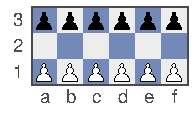
\includegraphics[width=\linewidth]{figures/dawson_strip.pdf}
\caption{}
\label{fig:dawson_strip}
\end{subfigure}\hfill
\begin{subfigure}{0.48\columnwidth}
\centering
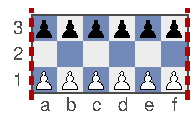
\includegraphics[width=\linewidth]{figures/dawson_ring.pdf}
\caption{}
\label{fig:dawson_ring}
\end{subfigure}
\caption{Starting position of Dawson's chess on six files. (a) Flat $3\times6$ strip (ordinary board).
(b) $3\times6$ cylinder; the arrow marks the seam, so files f and a are adjacent.}
\label{fig:dawson_boards}
\end{figure}

\begin{figure*}[!t]
\centering
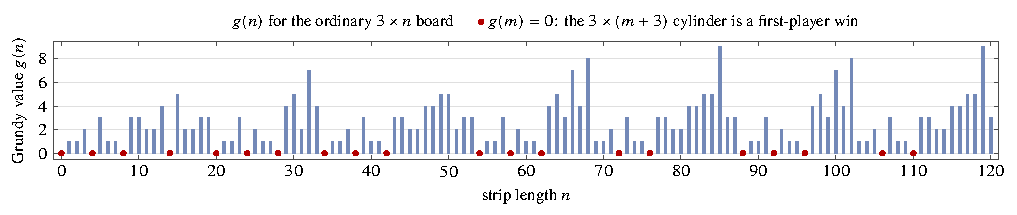
\includegraphics[width=\textwidth]{figures/dawson_grundy.pdf}
\caption{Grundy values $g(n)$ of Dawson's chess on the flat $3\times n$ board (octal game
$\mathbf{0.137}$) for $n\le120$. The dots (red) mark $g(m)=0$, where the flat $3\times m$ board is a
second-player win and the $3\times(m+3)$ cylinder is a first-player win (Theorem~\ref{thm:ring}).}
\label{fig:dawson_grundy}
\end{figure*}

\emph{Rules.} Dawson's chess~\cite{Dawson1935} is played on a $3\times n$ board
(Fig.~\ref{fig:dawson_boards}). White pawns fill rank~1, black pawns fill rank~3, and rank~2 is empty.
Pawns move and capture as in chess, and captures are compulsory. There is no room for a double step, so
there is no en passant, and no pawn ever promotes. Under normal play the last player to move wins. Dawson
himself posed the misère form, which we return to below.

Let us see what one move does. Call a file \emph{untouched} if it still has its white pawn on rank~1, its
black pawn on rank~3 and an empty square between them. Suppose white plays c1--c2 when the b- and d-files are
untouched. The pawn on c2 attacks b3 and d3, so black must capture, say b3$\times$c2. That pawn attacks b1 and d1,
so white must recapture, say d1$\times$c2. Black recaptures with d3$\times$c2 and white with b1$\times$c2. After the push and four
forced captures, the b- and d-files are empty, the c-file holds a blocked pair, and black is to move. Empty
and blocked files never change again, because a pawn can enter a file only by capturing on it. At the end of
a row the same push takes three plies and empties its one neighbor, and a push on a file with no untouched
neighbor is simply blocked.

So a strip of $n$ untouched files is a row of $n$ pins in which a move removes one pin together with its
surviving neighbors. This is the octal game $\mathbf{0.137}$ of Guy and Smith~\cite{GuySmith1956,WinningWays}.
Both players have the same moves, so the game is impartial and each strip has a Grundy value $g(n)$:
$g(0)=0$, $g(1)=1$ and, for $n\ge2$,
\begin{equation}\label{eq:dawson}
g(n)=\operatorname{mex}\bigl(\{g(n-2)\}\cup\{g(a)\oplus g(b) : a+b=n-3\}\bigr),
\end{equation}
where $g(n-2)$ comes from a push on an end file, $\oplus$ is the bitwise exclusive or, and mex is the least
non-negative integer not in the set. A board with several strips has the nim-sum of their values, and the
first player wins the flat $3\times n$ board if and only if $g(n)\ne0$. The values have period 34 with last
exception $n=51$~\cite{GuySmith1956}; we reproduced this for $n\le300$ with two programs \lab{C2}.

\emph{What was wrong.} In~\cite{Bhattacharjee2025} the game was a single row of pawns, and a pawn could be
removed only when both of its neighbors were empty. From a full row of two or more pawns no such move exists.
The recurrence given there, $G(n)=\operatorname{mex}\{G(a)\oplus G(b) : a+b=n-3\}$, omits the end-file
move and the value $g(1)=1$. It agrees with the true $g$ at only 31 of the 301 values $n=0,\dots,300$, and
the cylinder predictions built on it are wrong for 56 values of $n\le300$ \lab{C2}. The first is $n=4$. The
old recurrence gives $G(1)=0$ and predicts that the first player wins the $3\times4$ cylinder. In fact
white's push and its four captures leave one untouched file; black pushes that pawn, it is blocked, and
white has no move.

\begin{theorem}[Ring rule; \lab{P}, machine-checked for $n\le22$]\label{thm:ring}
On the full $3\times n$ cylinder with $n\ge3$, every first move, with its forced captures, leaves one strip
of $n-3$ untouched files with the opponent to move. Hence the cylinder has Grundy value
$\operatorname{mex}\{g(n-3)\}$, and the first player wins if and only if $g(n-3)=0$, that is, for
$n=3,7,11,17,23,27,31,37,41,45,57,\dots$
\end{theorem}

\begin{proof}
On a full ring every file has two distinct untouched neighbors, so every push starts the five-ply sequence
above. It ends with both neighbors empty, the pushed file blocked and the opponent to move. The other $n-3$
files are untouched and consecutive, and they are bounded on both sides by empty files that never change,
so they play as an ordinary strip. Up to rotation and color reversal every first move is the same, so the
cylinder has exactly one option.
\end{proof}

So the ring formula of~\cite{Bhattacharjee2025}, $\operatorname{mex}\{g(n-3)\}$, and its remark that the
ring's value is always 0 or 1, are right once the correct $g$ is used. Since $g$ is eventually periodic, so
is the ring's outcome. Fig.~\ref{fig:dawson_grundy} shows $g(n)$ for $n\le120$ and marks the zeros that
make the cylinder a first-player win.


\emph{Misère play.} In Dawson's own question the last player to move loses. Every forced sequence has odd
length and ends with the player who began it, so the reduction to $\mathbf{0.137}$ and the ring rule hold in
misère play too: the first player wins the misère cylinder if and only if the strip of $n-3$ files is a
misère P-position (a loss for the player to move). The cylinder is therefore exactly as hard as a single strip, and misère Dawson's chess is
still unsolved. Plambeck and Siegel computed partial misère quotients of this game~\cite{PlambeckSiegel2008}.
Our own implementation of their algorithm reproduces their quotient for strips of length at most 32 exactly,
of order 638 with 109 P-positions, and it agrees with exhaustive search on 7.4 million positions \lab{C2}.
The next quotient did not converge.

\emph{A warning about sums.} Our pawn games add up as sums of components, but Dawson's chess does not do
so board by board. If we compute the partizan value of the flat $3\times5$ board on its own, as we did for
pawn positions, we get $\star$, although $g(5)=3$; the outcome agrees, but the value cannot be added. Such a
computation lets a player answer in another component while a capture is pending, and the compulsory-capture
rule forbids that. The additive invariant is the Grundy value of the push together with its forced captures.
